\documentclass[11pt]{article}

\author{Math 123}
\date{Due March 10, 2023 by midnight} 
\title{Homework 6}

\usepackage{graphicx,xypic}
\usepackage{amsthm}
\usepackage{amsmath,amssymb}
\usepackage{amsfonts}
\usepackage{xcolor}
\usepackage[margin=1in]{geometry}
\usepackage[shortlabels]{enumitem}
\newtheorem{problem}{Problem}
\renewcommand*{\proofname}{{\color{blue}Solution}}


\usepackage{fancyhdr}
\pagestyle{fancy}
\rhead{Math 123, Homework 6}

\setlength{\parindent}{0pt}
\setlength{\parskip}{1.25ex}

% tikz
\usepackage{tikz}
\usetikzlibrary{intersections, angles, quotes, positioning}
\usetikzlibrary{arrows.meta}
\usepackage{pgfplots}
\pgfplotsset{compat=1.13}


\tikzset{
	force/.style={thick, {Circle[length=2pt]}-stealth, shorten <=-1pt}
}

% quiver style
\usepackage{tikz-cd}
% `calc` is necessary to draw curved arrows.
\usetikzlibrary{calc}
% `pathmorphing` is necessary to draw squiggly arrows.
\usetikzlibrary{decorations.pathmorphing}

% A TikZ style for curved arrows of a fixed height, due to AndréC.
\tikzset{curve/.style={settings={#1},to path={(\tikztostart)
					.. controls ($(\tikztostart)!\pv{pos}!(\tikztotarget)!\pv{height}!270:(\tikztotarget)$)
					and ($(\tikztostart)!1-\pv{pos}!(\tikztotarget)!\pv{height}!270:(\tikztotarget)$)
					.. (\tikztotarget)\tikztonodes}},
	settings/.code={\tikzset{quiver/.cd,#1}
			\def\pv##1{\pgfkeysvalueof{/tikz/quiver/##1}}},
	quiver/.cd,pos/.initial=0.35,height/.initial=0}

% TikZ arrowhead/tail styles.
\tikzset{tail reversed/.code={\pgfsetarrowsstart{tikzcd to}}}
\tikzset{2tail/.code={\pgfsetarrowsstart{Implies[reversed]}}}
\tikzset{2tail reversed/.code={\pgfsetarrowsstart{Implies}}}
% TikZ arrow styles.
\tikzset{no body/.style={/tikz/dash pattern=on 0 off 1mm}}

\begin{document}

\maketitle

% You are required to put your name here:
{\bf\Large Name: George Chemmala} 


\vspace{.3in}
Topics covered: vertex cuts, connectivity, Menger's theorem, network flows

Instructions: 
\begin{itemize}
\item This assignment must be submitted on Gradescope by the due date. 
\item If you collaborate with other students (which is encouraged!), please mention this somewhere on the assignment. 
\item If you are stuck, please ask for help (from me, a TA, a classmate). Use Campuswire!  
\item You may freely use any fact proved in class. In general, you should provide proof for facts used that were not proved in class. 
\item Please restrict your solution to each problem to a single page. Usually solutions can be even shorter than that. If your solution is very long, you should think more about how to express it concisely.
\end{itemize}

\pagebreak 


\begin{problem}
Let $G$ be a graph. 
\begin{enumerate}[(a)]
\item Give a counterexample to the following statement: If $e$ is a cut-edge of $G$, then at least one vertex of $e$ is a cut-vertex of $G$. \footnote{We did not define cut edge in class, but it means what you most likely guess.} 
\item Add a hypothesis to correct the above statement. 
\end{enumerate} 
\end{problem}

\begin{proof}
\begin{enumerate}
    \item[]
    \item[a] Let \(G\) be a graph attached to two vertices s.t.
% https://q.uiver.app/?q=WzAsNSxbMCwxLCJHIl0sWzEsMCwiXFxidWxsZXQiXSxbMSwyLCJcXGJ1bGxldCJdLFsyLDEsIlxcYnVsbGV0Il0sWzMsMSwiXFxidWxsZXQiXSxbMCwxLCIiLDAseyJzdHlsZSI6eyJoZWFkIjp7Im5hbWUiOiJub25lIn19fV0sWzAsMiwiIiwyLHsic3R5bGUiOnsiaGVhZCI6eyJuYW1lIjoibm9uZSJ9fX1dLFsxLDMsIiIsMCx7InN0eWxlIjp7ImhlYWQiOnsibmFtZSI6Im5vbmUifX19XSxbMywyLCIiLDAseyJzdHlsZSI6eyJoZWFkIjp7Im5hbWUiOiJub25lIn19fV0sWzMsNCwiYyIsMCx7InN0eWxlIjp7ImhlYWQiOnsibmFtZSI6Im5vbmUifX19XV0=
\[\begin{tikzcd}
	& \bullet \\
	G && \bullet & \bullet \\
	& \bullet
	\arrow[no head, from=2-1, to=1-2]
	\arrow[no head, from=2-1, to=3-2]
	\arrow[no head, from=1-2, to=2-3]
	\arrow[no head, from=2-3, to=3-2]
	\arrow["c", no head, from=2-3, to=2-4]
\end{tikzcd}\]

    Where the edge label \(c\) is the cut edge, but neither vertex connected to it is a cut vertex.

    \item[b] If $e$ is a cut-edge of $G$ connecting two vertices of degree greater than \(1\), then at least one vertex of $e$ is a cut-vertex of $G$. 
\end{enumerate}
\end{proof}

\pagebreak
\begin{problem}
Compute (with proof) $\kappa(u,v)$ for the graph below.
\begin{center}
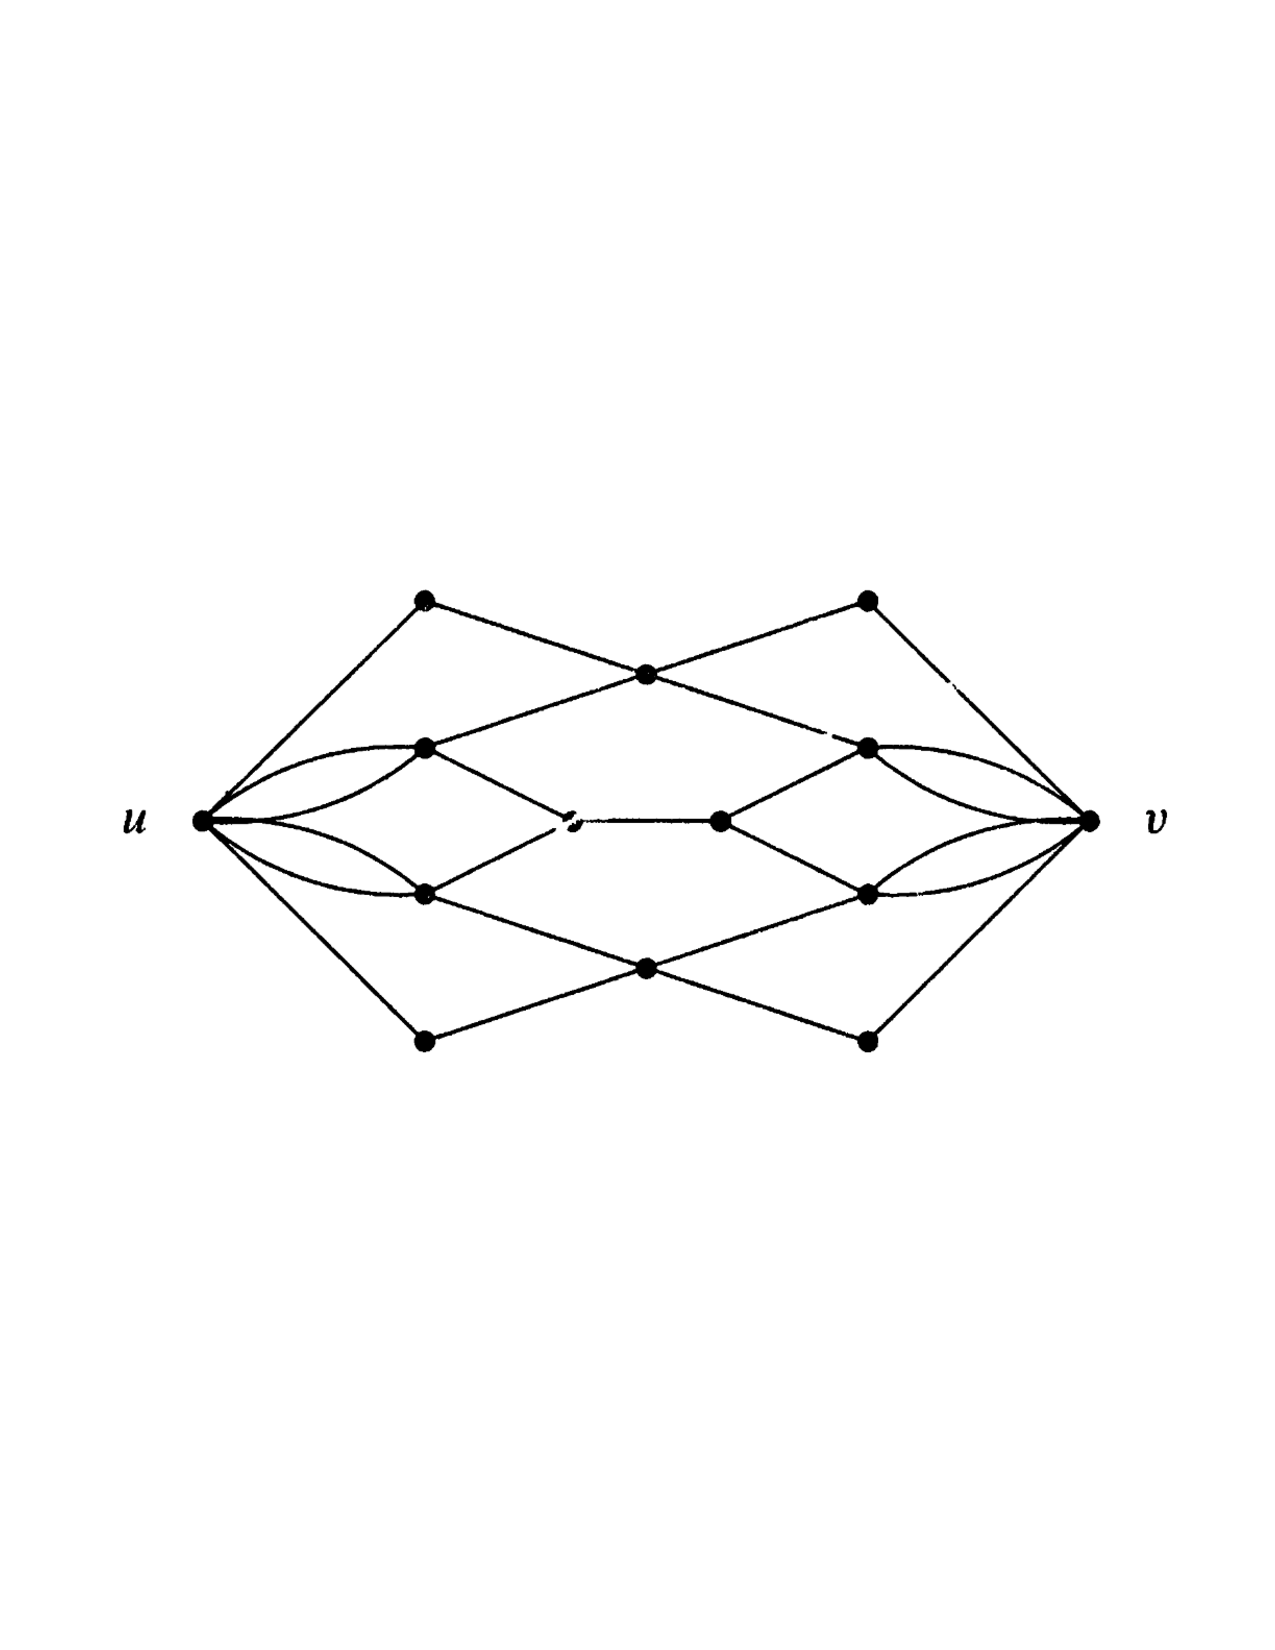
\includegraphics[scale=.4]{hw6-graph.pdf}
\end{center}
\end{problem}

\begin{proof}
% https://q.uiver.app/?q=WzAsMTQsWzAsMywidSJdLFsyLDIsIlxcYnVsbGV0Il0sWzIsNCwiXFxidWxsZXQiXSxbMiw2LCJcXGJ1bGxldCJdLFsyLDAsIlxcYnVsbGV0Il0sWzQsMSwiYSJdLFszLDMsImIiXSxbNCw1LCJjIl0sWzUsMywiXFxidWxsZXQiXSxbNiwwLCJcXGJ1bGxldCJdLFs2LDIsIlxcYnVsbGV0Il0sWzYsNCwiXFxidWxsZXQiXSxbNiw2LCJcXGJ1bGxldCJdLFs4LDMsInYiXSxbMCwxLCIiLDAseyJjdXJ2ZSI6LTEsInN0eWxlIjp7ImhlYWQiOnsibmFtZSI6Im5vbmUifX19XSxbMCwyLCIiLDIseyJjdXJ2ZSI6LTEsInN0eWxlIjp7ImhlYWQiOnsibmFtZSI6Im5vbmUifX19XSxbMCwzLCIiLDIseyJzdHlsZSI6eyJib2R5Ijp7Im5hbWUiOiJzcXVpZ2dseSJ9LCJoZWFkIjp7Im5hbWUiOiJub25lIn19fV0sWzAsNCwiIiwyLHsic3R5bGUiOnsiYm9keSI6eyJuYW1lIjoic3F1aWdnbHkifSwiaGVhZCI6eyJuYW1lIjoibm9uZSJ9fX1dLFs0LDUsIiIsMix7InN0eWxlIjp7ImJvZHkiOnsibmFtZSI6InNxdWlnZ2x5In0sImhlYWQiOnsibmFtZSI6Im5vbmUifX19XSxbMSw1LCIiLDAseyJzdHlsZSI6eyJoZWFkIjp7Im5hbWUiOiJub25lIn19fV0sWzEsNiwiIiwwLHsic3R5bGUiOnsiYm9keSI6eyJuYW1lIjoic3F1aWdnbHkifSwiaGVhZCI6eyJuYW1lIjoibm9uZSJ9fX1dLFsyLDYsIiIsMix7InN0eWxlIjp7ImhlYWQiOnsibmFtZSI6Im5vbmUifX19XSxbMiw3LCIiLDIseyJzdHlsZSI6eyJoZWFkIjp7Im5hbWUiOiJub25lIn19fV0sWzMsNywiIiwxLHsic3R5bGUiOnsiYm9keSI6eyJuYW1lIjoic3F1aWdnbHkifSwiaGVhZCI6eyJuYW1lIjoibm9uZSJ9fX1dLFswLDEsIiIsMSx7ImN1cnZlIjoxLCJzdHlsZSI6eyJib2R5Ijp7Im5hbWUiOiJzcXVpZ2dseSJ9LCJoZWFkIjp7Im5hbWUiOiJub25lIn19fV0sWzAsMiwiIiwxLHsiY3VydmUiOjEsInN0eWxlIjp7ImhlYWQiOnsibmFtZSI6Im5vbmUifX19XSxbNiw4LCIiLDAseyJzdHlsZSI6eyJib2R5Ijp7Im5hbWUiOiJzcXVpZ2dseSJ9LCJoZWFkIjp7Im5hbWUiOiJub25lIn19fV0sWzUsOSwiIiwwLHsic3R5bGUiOnsiYm9keSI6eyJuYW1lIjoic3F1aWdnbHkifSwiaGVhZCI6eyJuYW1lIjoibm9uZSJ9fX1dLFs1LDEwLCIiLDAseyJzdHlsZSI6eyJoZWFkIjp7Im5hbWUiOiJub25lIn19fV0sWzcsMTEsIiIsMCx7InN0eWxlIjp7ImhlYWQiOnsibmFtZSI6Im5vbmUifX19XSxbNywxMiwiIiwwLHsic3R5bGUiOnsiYm9keSI6eyJuYW1lIjoic3F1aWdnbHkifSwiaGVhZCI6eyJuYW1lIjoibm9uZSJ9fX1dLFs4LDEwLCIiLDEseyJzdHlsZSI6eyJib2R5Ijp7Im5hbWUiOiJzcXVpZ2dseSJ9LCJoZWFkIjp7Im5hbWUiOiJub25lIn19fV0sWzgsMTEsIiIsMSx7InN0eWxlIjp7ImhlYWQiOnsibmFtZSI6Im5vbmUifX19XSxbOSwxMywiIiwwLHsic3R5bGUiOnsiYm9keSI6eyJuYW1lIjoic3F1aWdnbHkifSwiaGVhZCI6eyJuYW1lIjoibm9uZSJ9fX1dLFsxMCwxMywiIiwwLHsiY3VydmUiOjEsInN0eWxlIjp7ImJvZHkiOnsibmFtZSI6InNxdWlnZ2x5In0sImhlYWQiOnsibmFtZSI6Im5vbmUifX19XSxbMTEsMTMsIiIsMCx7ImN1cnZlIjoxLCJzdHlsZSI6eyJoZWFkIjp7Im5hbWUiOiJub25lIn19fV0sWzEyLDEzLCIiLDAseyJzdHlsZSI6eyJib2R5Ijp7Im5hbWUiOiJzcXVpZ2dseSJ9LCJoZWFkIjp7Im5hbWUiOiJub25lIn19fV0sWzExLDEzLCIiLDAseyJjdXJ2ZSI6LTEsInN0eWxlIjp7ImhlYWQiOnsibmFtZSI6Im5vbmUifX19XSxbMTAsMTMsIiIsMCx7ImN1cnZlIjotMSwic3R5bGUiOnsiaGVhZCI6eyJuYW1lIjoibm9uZSJ9fX1dXQ==
\[\begin{tikzcd}
	&& \bullet &&&& \bullet \\
	&&&& a \\
	&& \bullet &&&& \bullet \\
	u &&& b && \bullet &&& v \\
	&& \bullet &&&& \bullet \\
	&&&& c \\
	&& \bullet &&&& \bullet
	\arrow[curve={height=-6pt}, no head, from=4-1, to=3-3]
	\arrow[curve={height=-6pt}, no head, from=4-1, to=5-3]
	\arrow[squiggly, no head, from=4-1, to=7-3]
	\arrow[squiggly, no head, from=4-1, to=1-3]
	\arrow[squiggly, no head, from=1-3, to=2-5]
	\arrow[no head, from=3-3, to=2-5]
	\arrow[squiggly, no head, from=3-3, to=4-4]
	\arrow[no head, from=5-3, to=4-4]
	\arrow[no head, from=5-3, to=6-5]
	\arrow[squiggly, no head, from=7-3, to=6-5]
	\arrow[curve={height=6pt}, squiggly, no head, from=4-1, to=3-3]
	\arrow[curve={height=6pt}, no head, from=4-1, to=5-3]
	\arrow[squiggly, no head, from=4-4, to=4-6]
	\arrow[squiggly, no head, from=2-5, to=1-7]
	\arrow[no head, from=2-5, to=3-7]
	\arrow[no head, from=6-5, to=5-7]
	\arrow[squiggly, no head, from=6-5, to=7-7]
	\arrow[squiggly, no head, from=4-6, to=3-7]
	\arrow[no head, from=4-6, to=5-7]
	\arrow[squiggly, no head, from=1-7, to=4-9]
	\arrow[curve={height=6pt}, squiggly, no head, from=3-7, to=4-9]
	\arrow[curve={height=6pt}, no head, from=5-7, to=4-9]
	\arrow[squiggly, no head, from=7-7, to=4-9]
	\arrow[curve={height=-6pt}, no head, from=5-7, to=4-9]
	\arrow[curve={height=-6pt}, no head, from=3-7, to=4-9]
\end{tikzcd}\]

By removing \(a,b,c\) we disconnect \(u\) and \(v\), and we have \(3\) unique disjoint \(u\), \(v\)-paths therefore, \(\kappa (u, v) = 3\) by Menger's theorem. 
\end{proof}

\pagebreak
\begin{problem}
Find (with proof) the smallest $3$-regular graph with $\kappa(G)=1$. \footnote{Hint: consider a 1-element vertex cut $S$. What does $G\setminus S$ look like? } 
\end{problem}

\begin{proof}
% https://q.uiver.app/?q=WzAsMTEsWzEsMCwiXFxidWxsZXQiXSxbMCwxLCJcXGJ1bGxldCJdLFsxLDEsIlxcYnVsbGV0Il0sWzEsMiwiXFxidWxsZXQiXSxbNCwwLCJcXGJ1bGxldCJdLFs0LDIsIlxcYnVsbGV0Il0sWzQsMSwiXFxidWxsZXQiXSxbNSwxLCJcXGJ1bGxldCJdLFs2LDIsIlxcYnVsbGV0Il0sWzIsMSwiXFxidWxsZXQiXSxbMywxLCJcXGJ1bGxldCJdLFswLDEsIiIsMCx7InN0eWxlIjp7ImhlYWQiOnsibmFtZSI6Im5vbmUifX19XSxbMSwyLCIiLDAseyJzdHlsZSI6eyJoZWFkIjp7Im5hbWUiOiJub25lIn19fV0sWzIsMCwiIiwwLHsic3R5bGUiOnsiaGVhZCI6eyJuYW1lIjoibm9uZSJ9fX1dLFszLDIsIiIsMCx7InN0eWxlIjp7ImhlYWQiOnsibmFtZSI6Im5vbmUifX19XSxbMywxLCIiLDAseyJzdHlsZSI6eyJoZWFkIjp7Im5hbWUiOiJub25lIn19fV0sWzUsNiwiIiwwLHsic3R5bGUiOnsiaGVhZCI6eyJuYW1lIjoibm9uZSJ9fX1dLFs2LDcsIiIsMCx7InN0eWxlIjp7ImhlYWQiOnsibmFtZSI6Im5vbmUifX19XSxbNyw0LCIiLDAseyJzdHlsZSI6eyJoZWFkIjp7Im5hbWUiOiJub25lIn19fV0sWzQsNiwiIiwwLHsic3R5bGUiOnsiaGVhZCI6eyJuYW1lIjoibm9uZSJ9fX1dLFs3LDUsIiIsMCx7InN0eWxlIjp7ImhlYWQiOnsibmFtZSI6Im5vbmUifX19XSxbMCw5LCIiLDAseyJzdHlsZSI6eyJoZWFkIjp7Im5hbWUiOiJub25lIn19fV0sWzksMywiIiwwLHsic3R5bGUiOnsiaGVhZCI6eyJuYW1lIjoibm9uZSJ9fX1dLFs0LDEwLCIiLDAseyJzdHlsZSI6eyJoZWFkIjp7Im5hbWUiOiJub25lIn19fV0sWzUsMTAsIiIsMCx7InN0eWxlIjp7ImhlYWQiOnsibmFtZSI6Im5vbmUifX19XSxbMTAsOSwiIiwwLHsic3R5bGUiOnsiaGVhZCI6eyJuYW1lIjoibm9uZSJ9fX1dXQ==
\[\begin{tikzcd}
	& \bullet &&& \bullet \\
	\bullet & \bullet & \bullet & \bullet & \bullet & \bullet \\
	& \bullet &&& \bullet && \bullet
	\arrow[no head, from=1-2, to=2-1]
	\arrow[no head, from=2-1, to=2-2]
	\arrow[no head, from=2-2, to=1-2]
	\arrow[no head, from=3-2, to=2-2]
	\arrow[no head, from=3-2, to=2-1]
	\arrow[no head, from=3-5, to=2-5]
	\arrow[no head, from=2-5, to=2-6]
	\arrow[no head, from=2-6, to=1-5]
	\arrow[no head, from=1-5, to=2-5]
	\arrow[no head, from=2-6, to=3-5]
	\arrow[no head, from=1-2, to=2-3]
	\arrow[no head, from=2-3, to=3-2]
	\arrow[no head, from=1-5, to=2-4]
	\arrow[no head, from=3-5, to=2-4]
	\arrow[no head, from=2-4, to=2-3]
\end{tikzcd}\]
This graph has 10 vertices, so now we only need to show that there is no graph that satisfies the condition with fewer vertices/edges.

In \(G\), a $3$-regular graph with $\kappa(G)=1$, let \(v\) be a cut vertex. The resulting components (of which there are at least 2) either contain 1 or 2 vertices that connected to \(v\). This implies that there exists a vertex \(u\) which was not connected to \(v\). Therefore, each component has \(\geq 4\) vertices. Since there are at least 2 components with at least 4 vertices, \(G\) has have had at least 9 vertices. And since a graph must have an even number of odd degree vertices the graph can only have \(10, 12, 14 \ldots\) vertices with \(10\) being the minimum.
\end{proof} 


\pagebreak
\begin{problem}
Fix $k\ge2$ and let $Q_k$ be the hypercube graph. Prove that for any pair of vertices $x,y$ there exist $k$ pairwise disjoint $(x,y)$-paths. 
\end{problem}

\begin{proof}
By induction:

\emph{Base Case:} \(k = 0\) Since there is one vertex there are \(0\) pairwise disjoint paths between any two vertices of the graph 


\emph{Inductive Step:} \(k \to k - 1\) Let's consider vertices of \(Q_k\) as \(\overset{k}{\overbrace{\mathbb{Z}_2 \times \ldots \times \mathbb{Z}_2}} = (\mathbb{Z}_2)^k\). 

If they share a value in the tuple then they are in a \(Q_{k-1}\) sub hypercube graph, and this is the \(k - 1\) case, so there are \(k - 1\) paths. We can get another one by going from \(x\) to its mirror vertex in the other \(Q_{k-1}\) sub hypercube graph and then traveling to \(y\)'s mirror vertex. Therefore, there are \(k\) paths.

If they share no values (corners of the hypercube) then we can start each \(i\)th path by adding a \(1\) to the \(i\)th place of the tuple and then adding \((1, 0 \ldots 0)\), \((0, 1 \ldots 0) \ldots (0, 0 \ldots 1)\) to so all the bits are fliped to travel to the other corner.
\end{proof}

\pagebreak
\begin{problem}
Use Menger's theorem to prove K\"onig's theorem: if $G=(X\sqcup Y,E)$ is bipartite the maximum size of a matching of $G$ is equal to the minimum size of a vertex cover of $G$. \footnote{Hint: consider graph $G'$ obtained by adding vertices $a,b$ to $G$ and connecting $a$ to every vertex of $X$ and $b$ to every vertex of $Y$. } 
\end{problem}

\begin{proof}
Consider the graph $G'$ obtained by adding vertices $a,b$ to $G$ and connecting $a$ to every vertex of $X$ and $b$ to every vertex of $Y$. Therefore, the matchings correspond the disjoint paths from \(a\) to \(b\) and the vertex cover corresponds to the connectivity of \(a\) and \(b\).

By removing \(a\) and \(b\) from the disjoint paths from \(a\) to \(b\) we get matchings from vertices in \(X\) to vertices in \(Y\) Therefore, there are at least as many matchings as disjoint paths. (max \# of matchings in \(G\) \(\geq\) \# of disjoint paths from \(a\) to \(b\))

By removing \(S\), an \(x,y\)-seperating set, the set must contain vertices that, in total, are connected to all edges in \(G\); therefore, \(S\) is a vertex cover over \(G\). (\# of vertices in the separating set \(\geq\) min \# of vertices in the vertex cover of \(G\))

By Menger's theorem, \# of disjoint paths from \(a\) to \(b\) = \# of vertices in the separating set, so max \# of matchings in \(G\) \(\geq\) \# of disjoint paths from \(a\) to \(b\) = \# of vertices in the separating set \(\geq\) min \# of vertices in the vertex cover of \(G\), proving K\"onig's theorem
\end{proof}


\pagebreak
\begin{problem}
Use the matrix-tree theorem\footnote{From the end of lecture 2/28} to prove Cayley's theorem.\footnote{Use a connection between the determinant and eigenvalues. It may help to first try to guess the form of the answer. For the love of algebra, do NOT compute any determinants!}
\end{problem}

\begin{proof}
	\[
		\begin{bmatrix}
			n-1 & ... &  -1 \\
			... & n-1, ... &  ... \\
			-1 & ...  &  n-1
		\end{bmatrix}
		=
		\begin{bmatrix}
			n & ... & 0 \\
			... & n, ... &  ... \\
			0 & ...  &  n
		\end{bmatrix}
		-
		\begin{bmatrix}
			1 & ... & 1 \\
			... & ... &  ... \\
			1 & ...  &  1
		\end{bmatrix}
	\]
	\[
		n I - 
		\begin{bmatrix}
			1 & ... & 1 \\
			... & ... &  ... \\
			1 & ...  &  1
		\end{bmatrix}
	\]
	using matrix diagonalization (which does not effect the determinant) we can find that
	\[
		P^{-1} 
		\begin{bmatrix}
			1 & ... & 1 \\
			... & ... &  ... \\
			1 & ...  &  1
		\end{bmatrix}
		P
		=
		\begin{bmatrix}
			n-1 & ... & 0 \\
			... & 0, ... &  ... \\
			0 & ...  &  0
		\end{bmatrix}	
	\]
	by knowing that there are \(n-1\) cofactors

	\[
		n I - 
		P^{-1} 
		\begin{bmatrix}
			1 & ... & 1 \\
			... & ... &  ... \\
			1 & ...  &  1
		\end{bmatrix}
		P
		=
		\begin{bmatrix}
			1 & ... & 0 \\
			... & n, ... &  ... \\
			0 & ...  &  n
		\end{bmatrix}	
	\]
	Which we find that the determinant is \(\overset{n -2}{\overbrace{n \cdot \ldots \cdot n}} = n^{n-2}\) by multiplying the elements in the diagonal. 
\end{proof} 


\end{document}